Energieversorgung\\
Die Elektronik des Dojos bezieht die Energie von einem Akkumulator. Verwendet wird ein Lithiumakkumulator der Marke Trustfire mit einer Nennspannung von $3.7V$. Der Akkumulator besitzt eine Kapazität von $600mAh$.\\

Entladevorgang\\ 
Der Akkumulator besitzt eine Nennspannung von $3.925V$ bei voller Kapazität und $????V$ \ref{test_Spannungsversorgung} wenn die Kapazität erschöpft ist. Aus dieser Spannung wird mit einem Linearregler des Types ????? eine $3.3V$ Spannungsversorgung erstellt. Mit dieser Versorgung wird die gesammte Elektronik gespiesen.\\

Ladevorgang\\
Der Akkumulator wird über die Spannungsversorgung des USB-Ports geladen. Ein Akkumulator-Management-Chip sorgt dabei für eine konstante Spannung von $4.1V$. Diese Spannung wird benötigt um den Akkumulator zu laden. Die Ladezeit beträgt $???h$ \ref{test_Ladezeit}. Somit ist es möglich, den Akkumulator über eine Nacht komplett zu laden. 


Um herauszufinden welche Leistung von der Energieversorung bereitgestellt wird, wurden einige Test durchgeführt.

Zuerst wurde die Messung ohne zusätzlichen Widerstand durchgeführt. Somit kann die Leerlaufleistung der Batterie bestimmt werden. Dies führte zu folgenden Werten:
\begin{equation}
I = 1.07mA
\end{equation}

\begin{equation}
U_{Ndl} = 3.295V
\end{equation}

\begin{equation}
U_{B} = 3.925V
\end{equation}
dabei ist $I$ der gemessene Srom, $U_{Ndl}$ ist die Spannung welche nach dem Linearregler gemessen wurde und $U_{B}$ ist die Batteriespannung. Somit beträgt die Leistung der Ladeschaltung im Leerlauf:
\begin{equation}
P_{LL}  = 4.199mW
\end{equation}

Die Messungen mit einem angeschlossenen Widerstand haben ergeben: \\

\begin{table}[hp]
\centering
\label{messungen_Energie}
\begin{tabular}{|l|c|c|c|}
\hline
Widerstand [$\Omega$]     & 100   & 50    & 10    \\ \hline
Batteriestrom [$mA$]    & 32.55 & 63.79 & 293.3 \\ \hline
Batteriespannung [$V$] & 3.823 & 3.735 & 2.979 \\ \hline
Widerstandsstrom [$mA$] & 31.06 & 62.03 & 278.1 \\ \hline
Ausgangsspannung [$V$]  & 3.293 & 3.292 & 2.95  \\ \hline
Leistung [$mW$]  & 0.124 & 0.238 & 0.874  \\ \hline
\end{tabular}
\end{table}

\subsection{Entladung und Laden}

Um herauszufinden wie lange das entladen bzw. das Laden der Batterie geht wurden einige Tests durchgeführt.

\subsection*{Entladen}
Um die Batterie zu entladen wurde eine $100\Omega$ Last angeschlossen und dabei ein Entladestrom von $70.6mA$ erreicht. Die Messungen wurden bis zur vollständigen Entladung vollzogen. 
In den Abbildungen \ref{fig:EntladekurveSpannung} und  \ref{fig:EntladekurveStrom} ist die Entladekurve für die Spannung sowie für den Strom abgebildet:

\begin{figure}[h]
	\centering
	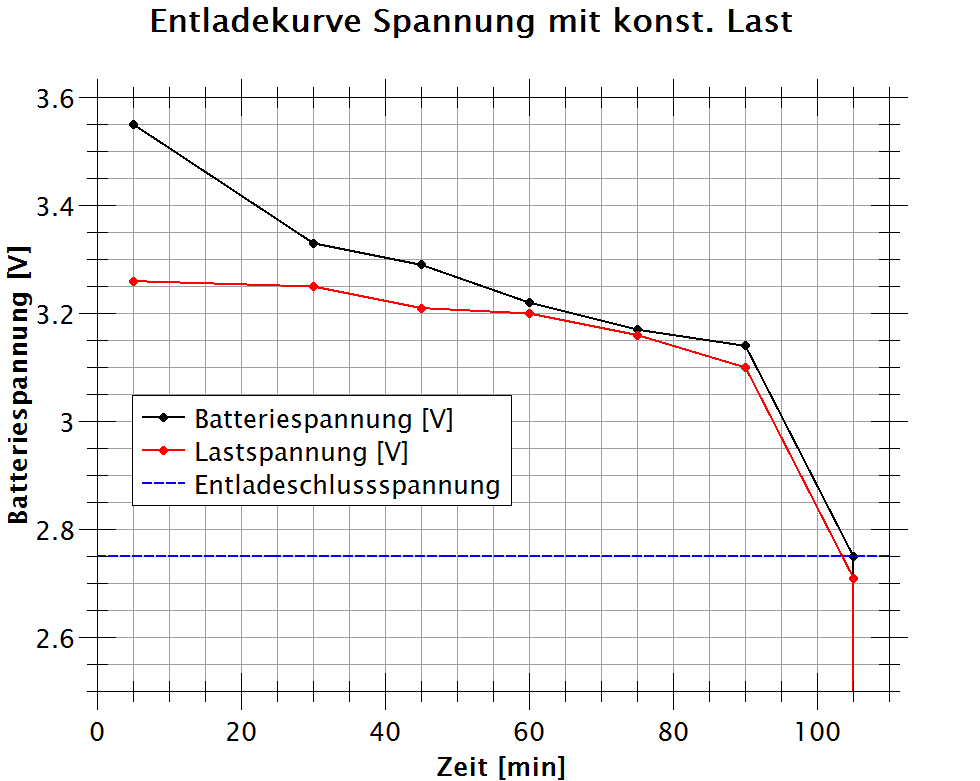
\includegraphics[width=\textwidth]{graphics/EnladekurveSpannung.png}
	\caption{Entladekurve bei einer Belastung von 100$\Omega$}
	\label{fig:EntladekurveSpannung}
\end{figure}

Wie in der Abbildung \ref{fig:EntladekurveSpannung} ersichtlich, hat die Batterie ein Tiefenentladungsschutz bei $2.75V$

\begin{figure}[htb]
	\centering
	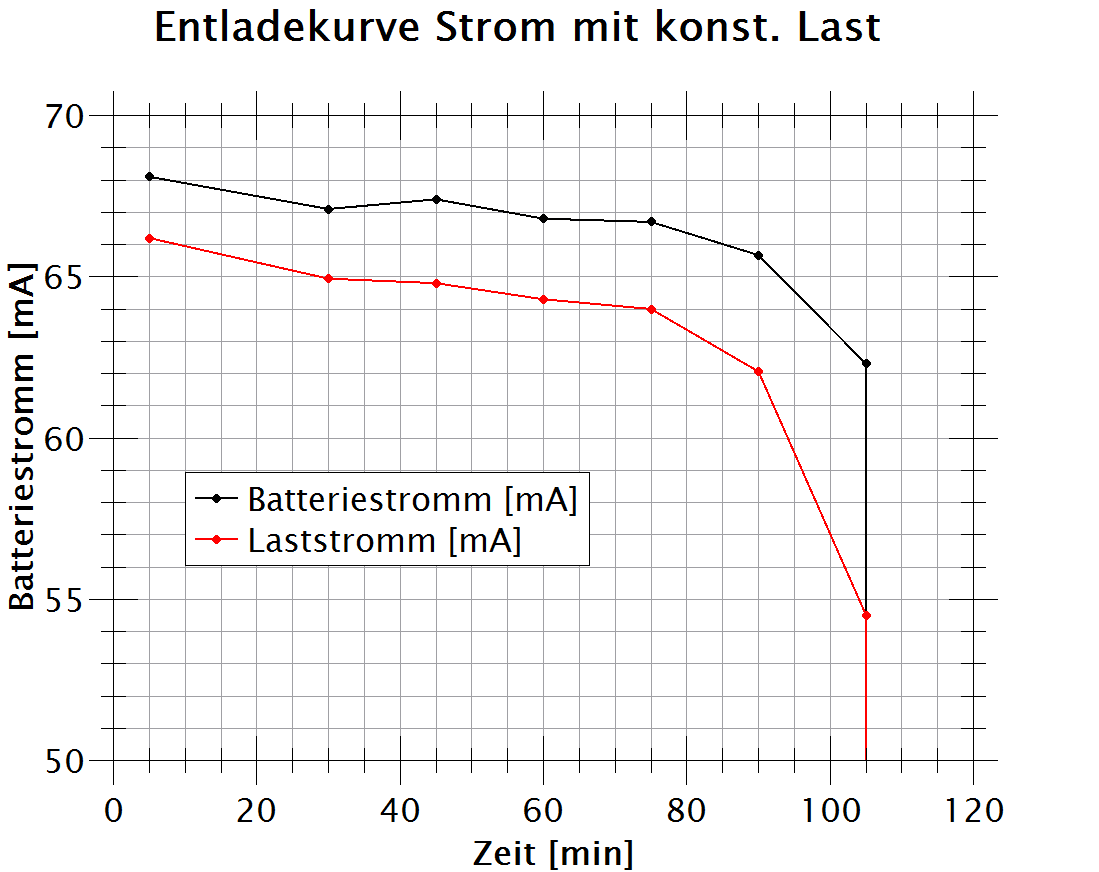
\includegraphics[width=\textwidth]{graphics/EnladekurveStrom.png}
	\caption{Entladekurve bei einer Belastung von 100$\Omega$}
	\label{fig:EntladekurveStrom}
\end{figure}



Die vollständige Entladung der Kurve dauerte $105min$. Dies sollte ausreichend sein, um den Dojo für $6000h$ zu betreiben.





\newpage

\subsection*{laden}
Beim aufladen der Batterie wurde eine Spannung von $4.22V$ verwendet. Dabei wurde vor dem anschliessen der Batterie ein Strom von $1.25mA$ gemessen. Die Ladekurve ist in der Abbildung\ref{fig:Ladeleistung} ersichtlich.

\begin{figure}[htb]
	\centering
	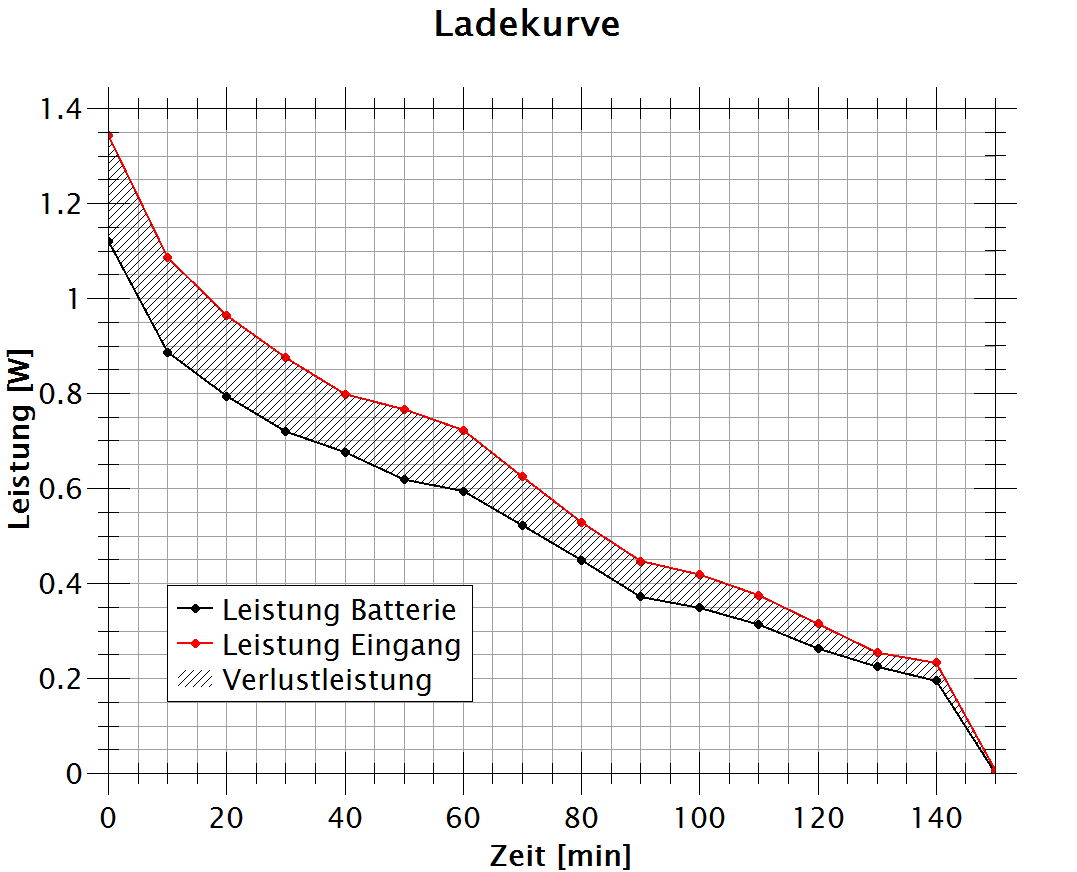
\includegraphics[width=\textwidth]{graphics/ladekurve.png}
	\caption{Ladekurve bei einer konstanten Eingangspannung 5V}
	\label{fig:Ladeleistung}
\end{figure}


Das komplette aufladen der Batterie dauerte $150min$. Somit kann das Museum den Dojo über Nacht problemlos aufladen.